\documentclass[12pt,a4paper,oneside,
	listof=totoc, % list of figures and list of tables in table of contents
	bibliography=totoc, % bibliography in table of contents
	%parskip=half, % half line between paragraphs instead of indentation
	BCOR=4mm,
	DIV=12,
]{scrartcl}


% -- Packages --------------------------------------------------------%
\usepackage{../template/report-settings}
\usepackage{mathtools}
\usepackage{booktabs}
\usepackage{float}
\usepackage{multirow,tabu} % tabular stuff like rowfont
\usepackage{algorithm,algpseudocode}
\usepackage{graphicx}
\usepackage{cleveref}
\usepackage{eurosym}
%\usepackage[left=5cm]{geometry}


% -- Settings --------------------------------------------------------%
\setLogo{../template/logo_i2ths}
\allowdisplaybreaks

% -- Shortcuts -------------------------------------------------------%
\newcommand*{\tb}[1]{\textbf{#1}}
\newcommand*{\ti}[1]{\textit{#1}}

% -- Own commands ----------------------------------------------------%
\newcommand*{\jquote}[1]{$\lceil$#1$\rfloor$}
\newcommand*{\myhline}{\bigskip\noindent\hrulefill\bigskip}
\newcommand*{\emptyline}{\vspace{\baselineskip} \\ \noindent}

% -- Cleveref specials -----------------------------------------------%
\crefname{constr}{constraint}{constaints}
\creflabelformat{constr}{#2{\upshape(#1)}#3}


% -- Document --------------------------------------------------------%
\begin{document}
	
	% Title page and Lists
	\pagenumbering{Roman}
	
	%-------------------------------------------------------------------------%
	%					Title
	%-------------------------------------------------------------------------%
	\begin{titlepage}
		\small
		\vspace*{4mm}%
		\parindent0pt%
		\begin{center}
			\bfseries This work was submitted to\\
			Computer Science Chair Informatik 2: Theory of hybride systems
		\end{center}
		\vspace*{25mm}
		\normalsize	
		\begin{center}
			\Large
            {\bfseries\sffamily Shortest Cable Routing of Heliostats in Solar Tower Power Plants}
			\\[20mm]
			\large
			Lab course report\\ Computer Science
		\end{center}
		\vfill
		\begin{center}
		\large August 2018
		\end{center}
		\vfill
	
	\begin{tabbing}
		\hspace*{4cm}\=\kill
		Presented by
		\> Duc Thanh Tran \\
		\> Matrikelnummer: 313 928 \\
		\> duc.thanh.tran@rwth-aachen.de \\[3mm]
																		
                                                                        
    	First supervisor
    	\> Prof. Dr. Ábrahám \\
    	\> Lehrstuhl II für Mathematik\\
    	\> RWTH Aachen University\\[3mm]
        
		Second supervisor
		\> Jun.-Prof. Dr. Christina Büsing\\
		\> Lehrstuhl II für Mathematik\\
		\> RWTH Aachen University\\[3mm]
        	
		Co-supervisor
		\> Dr. rer. nat. Pascal Richter\\
		\> Lehr- und Forschungsgebiet: Kontinuierliche Optimierung (IGPM)\\
		\> RWTH Aachen University
	\end{tabbing}

	\end{titlepage}
	
	
	
	%-------------------------------------------------------------------------%
	%					Declaration
	%-------------------------------------------------------------------------%
	\section*{Eigenst\"andigkeitserkl\"arung}
	Hiermit versichere ich, dass ich diesen Praktikumsreport selbst\"andig verfasst und keine anderen als die angegebenen Quellen und Hilfsmittel benutzt habe. Die Stellen meiner Arbeit, die dem Wortlaut oder dem Sinn nach anderen Werken entnommen sind, habe ich in jedem Fall unter Angabe der Quelle als Entlehnung kenntlich gemacht. Dasselbe gilt sinngem\"a\ss ~f\"ur Tabellen und Abbildungen. Diese Arbeit hat in dieser oder einer \"ahnlichen Form noch nicht im Rahmen einer anderen Pr\"ufung vorgelegen.
	\vspace{6mm}
	\begin{flushright}
	Aachen, im August 2018
	\\[12mm]
	Tran
	\end{flushright}
	\newpage

	\tableofcontents\clearpage
	
	% Sections
	\pagenumbering{arabic}
  	\section{Introduction}
In this work we present two heuristics that compute valid solutions to an optimization problem regarding a cabling problem in solar tower power plants. Such a plant focuses sunlight with the help of heliostats onto a receiver that is installed at the top of the solar tower. This energy heats up a medium like oil or sodium in order to power a turbine which generates electric energy in return.
Such a plant consists of a solar tower and heliostats that have to be connected to the solar tower with two types of cables, namely a power and data cable. Both cables are needed at each heliostat as the sun's position has to be taken into account for an efficient exploitation of solar energy. Regarding the cabling we have several limitations with respect to connectivity and planarity constraints. First, cables have restrictions regarding their maximum lengths between heliostats. Moreover, there are capacity constraints for each cable, namely that cables can only connect so many heliostats. Second, the planarity constraint is enforced in order to have a low maintenance cost when digging up trenches.
\emptyline
\noindent
Another source of energy is utilized in offshore wind farms for which the cabling problem has been studied in \cite{gonzales_2012,bauer_2015,fischetti_2018}. The same constraints like planarity are also present in their cabling problem. Our work builds up on two bachelor's theses that studied the solar tower power plants \cite{franziska_2017,tanja_2018}.
\emptyline
\noindent
In the following we will give a formal definition of our problem and present two heuristics that apply the local search optimization method \cite{aarts_2003,voss_2012}. This approach was chosen due to the high complexity of the cabling problem, which is especially difficult to solve for large instances that inhibit a lot of heliostats. Then, an evaluation part is followed where we have applied both heuristics onto the PS10 solar tower power plant \cite{osuna_2001,osuna_2006}. Afterwards we give a short summary and possible future work.



  	\newcommand*{\trenchcost}{c^\text{trench}}
% DATA CABLE
\newcommand*{\datacost}{c_d^\text{data}}
\newcommand*{\datatotalcost}{c_{d,vw}^\text{data}}
\newcommand*{\datalength}{L_d^\text{data}}
\newcommand*{\datacapacity}{M_d^\text{data}}
% SWITCHES
\newcommand*{\switchcosts}{c_{s}^\text{lcu}}

\section{Problem statement}
Formally, we are given an undirected graph $G=(V,E)$ where $V=\{T\} \cup V_H$ with $T$ being our solar tower and $V_H:=\{v_1,\ldots,v_{n}\}$ denotes the set of heliostats. Note that we work in a metric space $(\mathbb{R}^2,d)$, thus we denote with $v_x\in\mathbb{R}$ and $v_y \in\mathbb{R}$ both coordinates for each vertex $v\in V$. Moreover, the metric is simply the euclidean distance 
\begin{equation}
  d(v,w) := \sqrt{(v_x-w_x)^2 + (v_y-w_y)^2} \nonumber
\end{equation}
between nodes $v,w\in V$. In other words, each vertex $v\in V$ has a specified position in a 2D plane.
\emptyline
\noindent
Before a cable can be installed a trench has to be constructed by workers for which we have to pay installation costs. Let us denote these costs per meter with $\trenchcost\in\mathbb{R}^+$. In other words, the total costs of providing a trench between $v,w\in V$ is \\ 
$c_{vw}^\text{trench} := d(v,w)\cdot\trenchcost$.


\subsection{Data cable and local control units}
  We can install different types of cables which have length and connection restrictions depending on its type. For this matter let $D$ be the set of data cables with costs $\datacost\in\mathbb{R}^+$ per meter for each cable $d\in D$. We further define for readability the costs $\datatotalcost:=d(v,w)\cdot \datacost$ of installing a cable of type $d$ on the edge $vw\in E$. Furthermore, each data cable $d\in D$ has a length restriction $\datalength\in\mathbb{R}^+$ and a restriction on how many heliostats it can connect to, that is, $\datacapacity\in\mathbb{N}$ for $d\in D$.
  \emptyline
  Aside from the cables we have to build \emph{local control units} (LCU) at each heliostat. These LCUs are used for communication processing and may allow branching by e.g. installing an 8- or 16-port LCU at an heliostat. Each of these LCU has connectivity-restrictions for each cable type $d\in D$. For this matter, let $S$ the set of all LCUs where each $s\in S$ has installation costs $\switchcosts\in\mathbb{R}^+$. The connectivity or vertex-degree restrictions are given by $l_{s,d}, u_{s,d}\in\mathbb{N}$ for each LCU $s\in S$ and cable type $d\in D$. Both restrictions state that the LCU $s\in S$ has to connect at least $l_{s,d}$ cables of type $d\in D$, whereas $u_{s,d}$ is the upper bound of incident cables of type $d\in D$ at an heliosat that installed LCU $s\in S$.

  

\subsection{Power cables}
\ToDo{formal definition}

\subsection{Cabling problem}
\begin{tcolorbox}
\label{prob:cabling_problem}
\begin{problem}[Cabling Problem]
  Given a complete, undirected graph $G=(V,E)$.
\end{problem}
\end{tcolorbox}

\ToDo{capacity constraint}


    \section{Data}
We present real world data regarding costs per meter for various data as well as power cables. Moreover, many different LCUs and trench/installation costs are provided for which we can test our heuristics on. The experiments are running on the PS10 solar tpower power plant instance \cite{osuna_2001,osuna_2006} for which the coordinates are provided, a sketch of this instance can be seen in \cref{fig:ps10}.

\begin{figure}[H]
  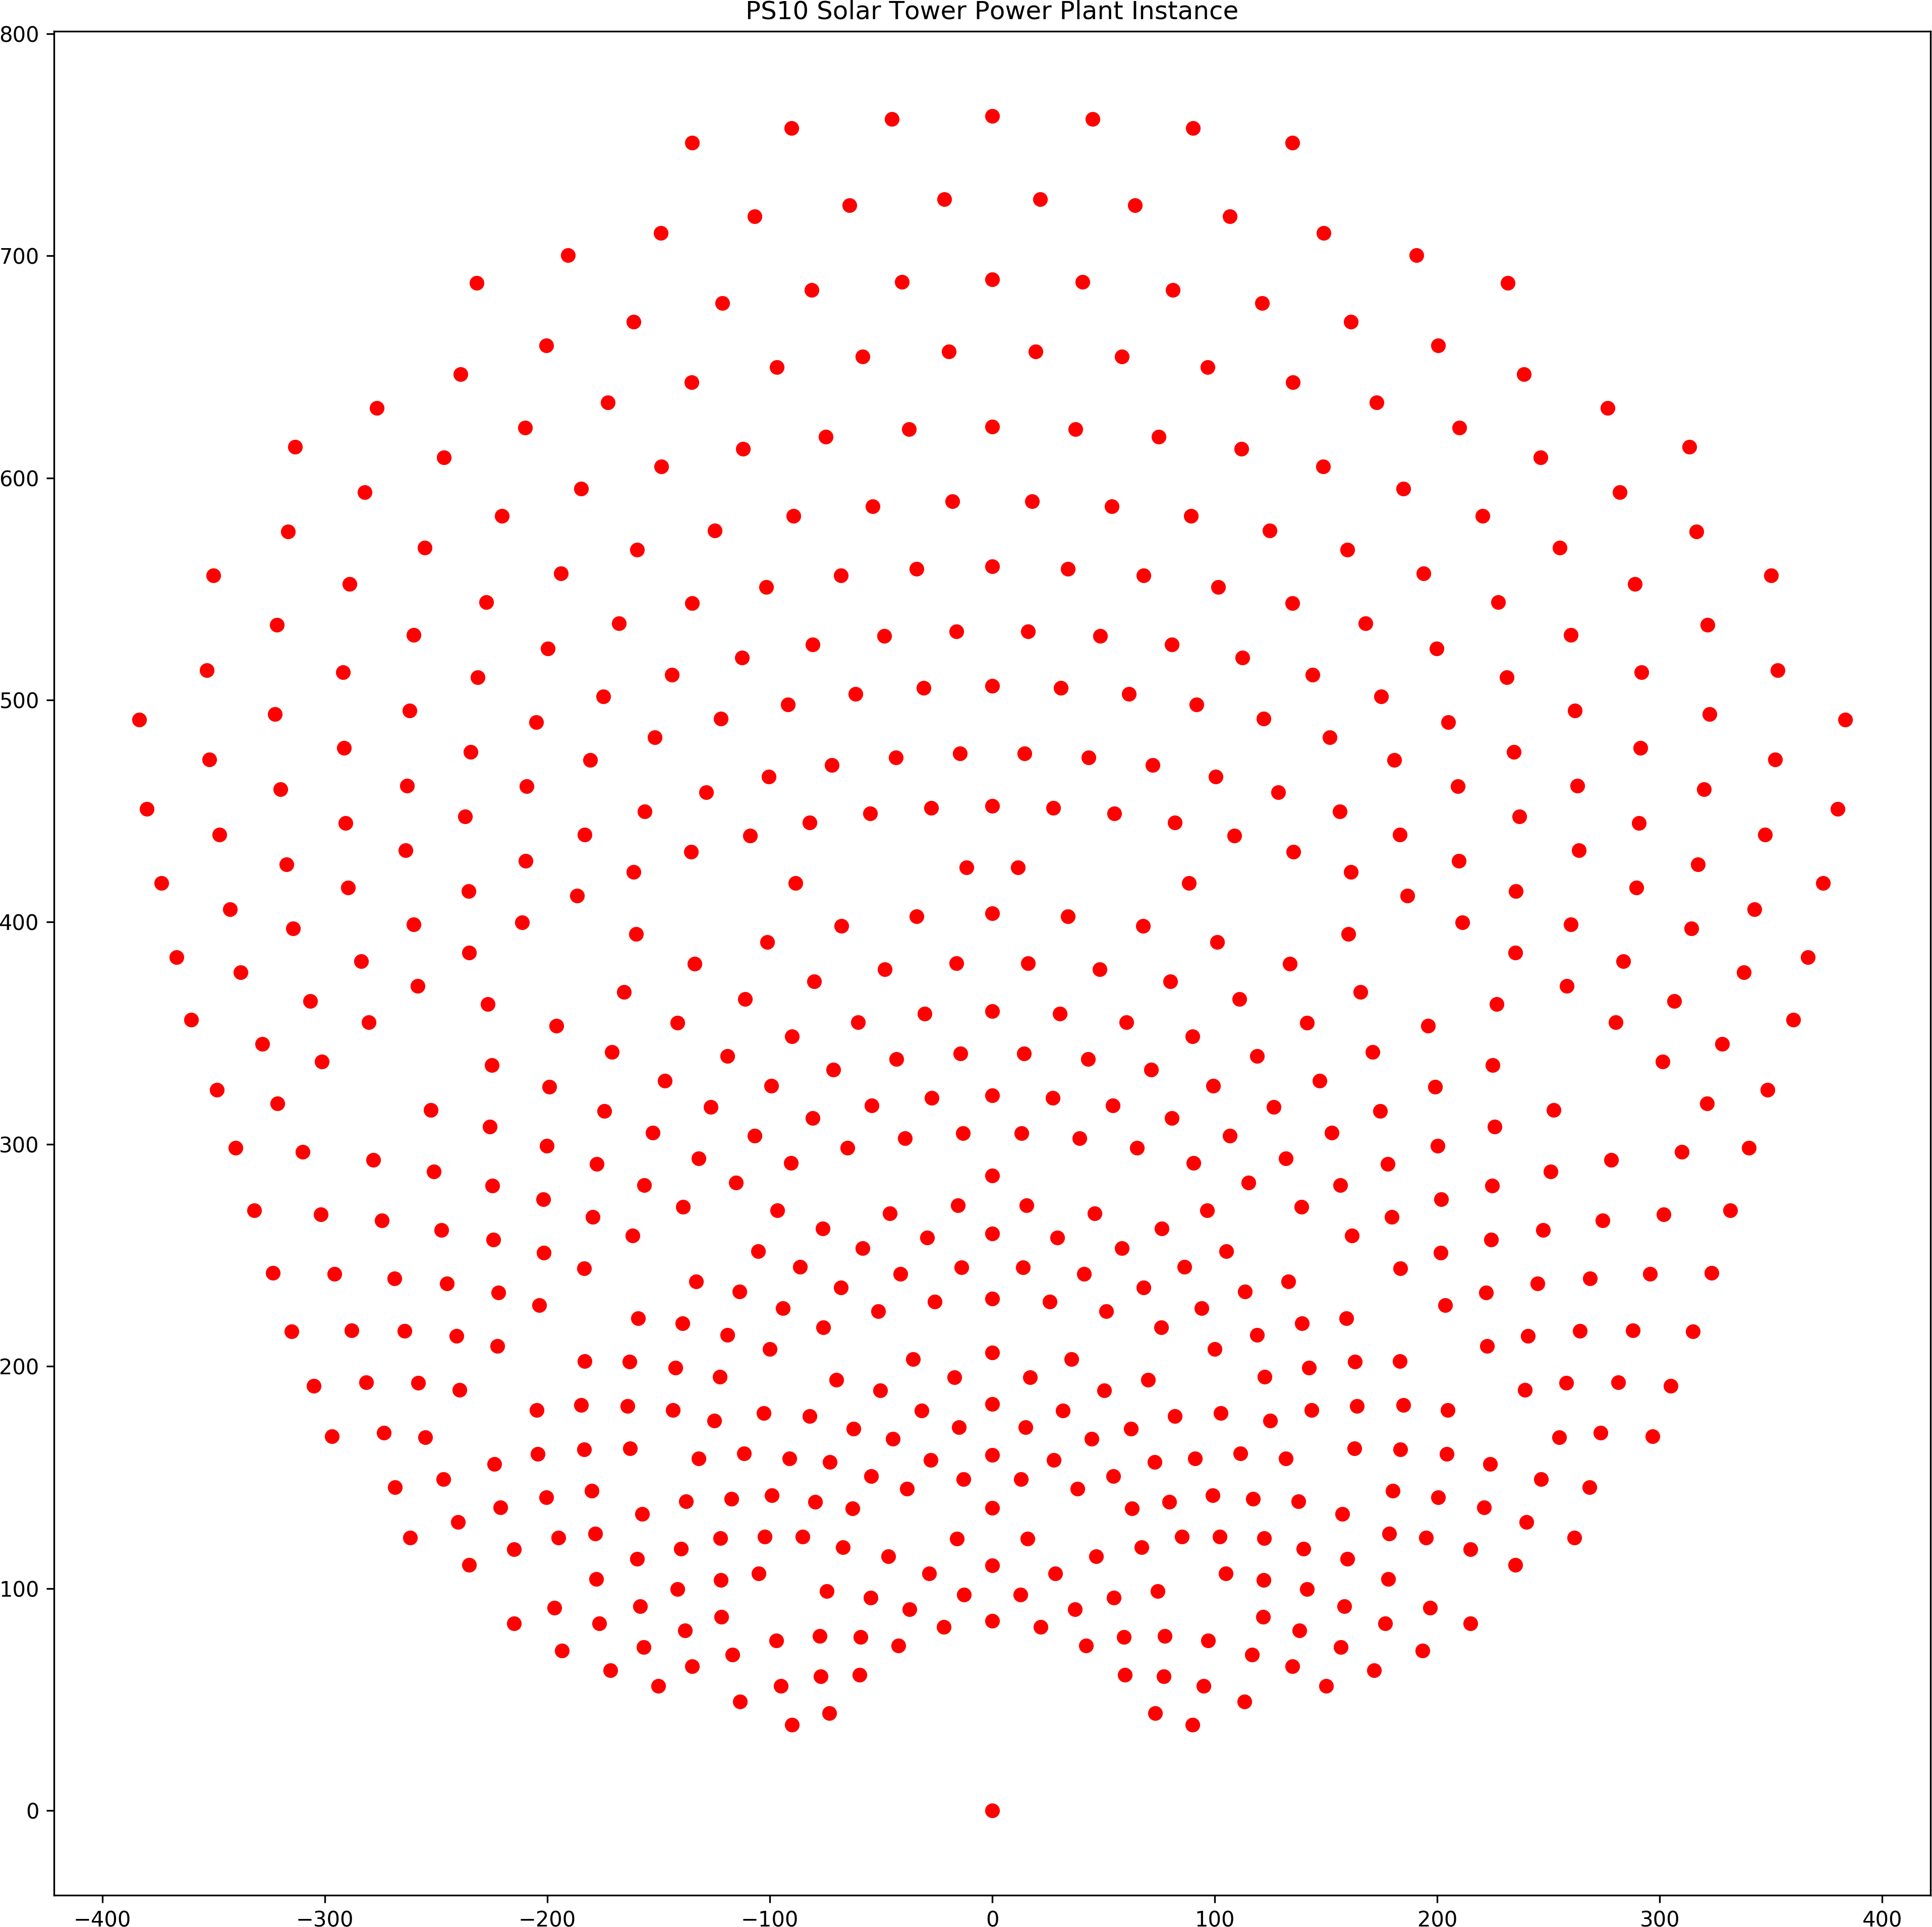
\includegraphics[width=\linewidth]{./img/ps10_instance.png}
  \caption{PS10 instance with its heliostats and the solar tower at coordinate $(0,0)$.}
  \label{fig:ps10}
\end{figure}

\subsection{Trench costs}
For the trench costs we are considering four different costs, each depending on the country we are located in. Each trench has to be constructed by workers and has a depth of 1m as well as 1m in width and length.
  \begin{table}[H]
    \caption{Trench costs for different countries}
    \label{tab:data:trench}
    \begin{center}
    \begin{tabular}{l|c}
      Country & Costs [\euro/m] \\
      \midrule
      Australia & 50 \\
      Spain & 25 \\
      South Africa & 10 \\
      United Arab Emirates & 10
    \end{tabular}
    \end{center}
  \end{table}

\subsection{Data Cable}
  Regarding the data cable we are able to install either a copper or fiberglass cable. The copper cable is much cheaper however it has harsh restrictions regarding its usage, making it only usable for endpoint connections. The fiberglass on the other hand can connect an arbitrary amount of heliostats and has no length restrictions.
  \begin{table}[H]
  \caption{Possible data cables with their cost and restrictions.}
  \label{tab:data:cable}
  \begin{center}
    \begin{tabular}{l|cc|c}
      Data cable type & Max. capacity &  Max. length [m] & Price [\euro/m] \\
      \midrule
      Copper & 2 & 100 & 0.7\\
      Fiberglass & $\infty$ & $\infty$ & 2
    \end{tabular}
  \end{center}
\end{table}

\subsubsection{Local Control Units}
  Exactly one local control units is installed at every heliostat so that communication is enabled. All LCUs with the exception of an endpoint has exactly one ingoing fiberglass cable. The endpoint has exactly one ingoing copper cable.
  \begin{table}[H]
  \caption{Local control units with their degree and cable restrictions for both cable types.}
  \label{tab:data:lcu}
  \begin{center}
    \begin{tabular}{lc|cc|cc}
      LCU type $s$ & Price [\euro/piece] & \multicolumn{2}{c|}{Copper} & \multicolumn{2}{c}{Fiberglass} \\
      && $l_{s,\text{COPPER}}$ & $u_{s,\text{COPPER}}$ & $l_{s,\text{FIBER}}$ & $u_{s,\text{FIBER}}$\\
      \midrule
      Endpoint & 10 & 1 & 1 & 0 & 0 \\
      Conductor & 100 & 0 & 0 & 1 & 2 \\
      8-port copper & 800 & 0 & 7 & 1 & 2 \\
      8-port fiberglass & 800 & 0 & 0 & 1 & 9 \\
      16-port copper & 1500 & 0 & 15 & 1 & 2 \\
      16-port fiberglass & 1500 & 0 & 0 & 1 & 17 \\
    \end{tabular}
  \end{center}
  \end{table}
  Therefore, an 8-port copper LCU for example has up to 7 'outgoing' copper connections and up to one 'outgoing' fiberglass one.

\subsection{Power Cable}
The power cables are not restricted with LCUs. However, maximum capacity constraints have to be taken into account --- as opposed to glasfiber cables that do not have any capacity restrictions. Hence, we have to use more than one power cable for instances with more than 250 heliostats. Therefore we have to partition the heliostats field into partitions that is non-trivial. A simple heuristic is presented in \cref{sec:partitioning}.
\begin{table}[H]
  \begin{center}
  \caption{Power cables with their connectivity limitations and prices.}
  \begin{tabular}{l|cc|c}
    Power cable type & Max. capacity & Max. length [m] & Price [\euro/m] \\
    \toprule
    NYY-J 3x2.5 RE & 56 & 38.36 & 0.58 \\
    NYY-J 3x4 RE & 73 & 47.08 & 0.87 \\
    NYY-J 3x6 RE & 92 & 56.04 & 1.24 \\
    NYY-J 3x10 RE & 124 & 69.30 & 1.95 \\
    NYY-J 3x16 RE & 162 & 84.87 & 3.13 \\
    \midrule
    NYY-J 3x25 RM & 209 & 102.79 & 5.19 \\
    NYY-J 3x35 RM & 250 & 120.31 & 6.90
  \end{tabular}
  \end{center}
\end{table}
    \section{Heuristics}
In the following both sections we present our heuristics that are based on the local-search optimization method \cite{aarts_2003,voss_2012}. The basic structure of such an algorithm is shown in \cref{alg:local_search}. Basically we first compute an initial solution from the input and afterwards improve it stepwise until some stopping criterion is met. In principle the stepwise improvements are performed locally to $sol$ such that each step yields a valid solution to our optimization problem. 
\begin{algorithm}[H]
\caption{A general framework of a local search heuristic.}
\label{alg:local_search}
\begin{algorithmic}[1]
  \Procedure{Local-Search}{$input$}
    \State $init$ := \Call{Compute-Initial-Solution}{$input$}
    \State $sol := init$
    \While{stopping criterion not met}
      \State x := \Call{Compute-Next-Neighbor-Solution}{$sol$}
      \If{$c(x) < c(sol)$}
        \State $sol := x$
      \EndIf
    \EndWhile
    \State \Return $sol$
  \EndProcedure
\end{algorithmic}
\end{algorithm}
One may interpret this by jumping from one point in the valid solution search space to another one in a certain local neighborhood. This interpretation is depicted in \cref{fig:local_search_illustration} where $s_0$ is the initial solution that we improve in a stepwise-manner by selecting a neighboring solution $s_1$ in its neighborhood $N(s_0)$. Obviously $s_1$ has lower total costs than $s_2$, however, depending on the neighborhood size $|N(s_0)|$ it may be a computationally demanding task. Therefore, while generating the neighboring solutions in $N(s_0)$ we terminate the search process as soon as we encounter a solution $s_1\in N(s_0)$ with $c(s_1) < c(s_0)$. This search strategy is called \emph{first-improvement} as we do not generate the best neighboring solution but are satisfied with any kind of improvement. This process is then continued until some stopping criterion is met. In particular, one may terminate after $i\in\mathbb{N}$ steps or in our case terminate as soon as $N(s_i)$ does not yield any improving solution, hence $s_i$ is called \emph{locally optimal}.
\begin{figure}[H]
  \centering
  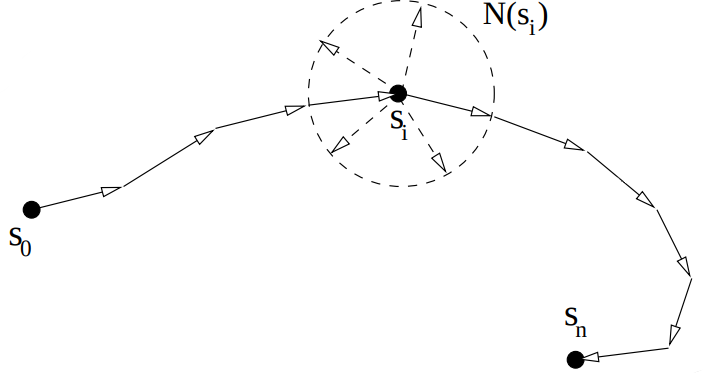
\includegraphics[width=0.7\linewidth]{./img/local_search.png}
  \caption{The search space where each point describes a valid solution to our optimization problem. We start from the initial solution $s_0$ improve it stepwise. For this matter we consider 'neighboring' solutions in $N(s_i)$ at the current solution $s_i$. When no neighboring solution is improving (i.e. has less total costs than current solution) we terminate our algorithm as $s_n$ is a locally optimal solution.}
  \label{fig:local_search_illustration}
\end{figure}

\ToDo{both cable in one, assign power automatically}

\subsection{Minimum Spanning Tree Approach}
The fact that each heliostat has to be connected to the solar tower $T$ with minimal costs infers utilizing a minimum spanning tree approach. We just need to consider the additional constraints of planarity as well as connectivity constraints. We thus choose Prim's algorithm \cite{prim_1957,cormen_2009} to compute an initial, valid solution to our problem. For the local search improvement steps we choose the \emph{cycle-neighborhood} function
\begin{equation*}
  N(T) := \{\tilde{T}\in\mathcal{T}|\}
\end{equation*}

    \section{Evaluation}
\ToDo{intial cost, diff: hamiltonian-power is done after LS}
\begin{table}
  \caption{Total cost and cable length after the local search algorithms.}
  \begin{center}
  \begin{tabular}{l|cc}
    & Total cost [\euro] & Total cable length [m] \\
    \toprule
    MST approach & 0 & 0 \\
    Hamiltonian path approach & 0 & 0\\
  \end{tabular}
  \end{center}
\end{table}
    \section{Conclusion}
The cabling problem asks the question of finding two spanning trees with length as well as capacity constraints onto the data and power cables. In particular, this problem has its origins from the cabling of solar tower power plants. Due to these additional constraints we are not able to solve the cabling problem in reasonable time, especially for big instances. Therefore we have designed two local search heuristic approaches that compute valid solutions within several hours for the instance PS10 that inhibits around 600 heliostats.

Besides, a partitioning problem arises due to capacity restrictions of power cables, that is, we have to install multiple power cables if the highest capacity is not sufficient to connect all heliostats. This problem is circumvented by computing a heuristic partition-solution, namely sorting angles of the solar tower and a respective heliostat and splitting the heliostat into equal-sized fields.
\emptyline
The first one has its basis from the minimum spanning tree, that is, the initial solution is computed by a modified version of Prim's algorithm, which takes switch installation costs into account. The local search utilizes the cycle neighborhood in addition to possible down-/upgrades of the power cables which beforehand have been computed greedily by considering capacities and length restrictions.

The second approach exploits the fact that switch costs are the main cost-factor, therefore Hamiltonian paths are considered. We first construct Hamiltonian paths greedily that is afterwards improved by a local search procedure which takes a triangulation-neighborhood into account.

\ToDo{evaluation results}
The Hamiltonian path achieves a total cost of xxxx \ToDo{cost} \euro compared 
\emptyline
In future work, one may consider multiple initial solutions, that are for example randomly generated, thereby enlarging the total search space of our procedure. Also, bigger neighborhoods could be considered in order to improve solution quality, however a heuristic search within the respective neighborhood may be necessary in order to select an improving neighboring solution. 

Moreover, we have left out the copper cables completely in order to simplify the heuristics because glasfiber cables do not inhibit any length or capacity restrictrions.


	
	% Bibliography
	\clearpage
	\bibliography{literature}
	
\end{document}
%---------------------------------------------------------------------------%
